\documentclass[
a4paper,
oneside,
listof=totoc,
plainfootsepline,
headsepline,
footsepline,
openbib,
numbers=noenddot
]{scrreprt}

\areaset{15cm}{26cm}

\usepackage[ngerman]{babel}
\usepackage{hyperref}
\usepackage[latin1]{inputenc}
\usepackage{eurosym}
\usepackage{graphicx}
\usepackage{pdflscape}
\usepackage{siunitx}

%set up minted for normal use and longlisting
\usepackage{caption}
\usepackage[chapter]{minted}
\newenvironment{longlisting}{\captionsetup{type=listing,belowskip=12pt}}{}
\setminted{breaklines=true}

\usepackage[backend=biber,citestyle=numeric,natbib=true]{biblatex} % Use the biber backend with the authoryear citation style (which resembles APA)

\addbibresource{literatur.bib} % The filename of the bibliography
%\bibliographystyle{unsrt}

\title{Projektdokumentation Homeserver}
\author{Thilo Wendt}

\begin{document}

\maketitle

\begin{abstract}
  Zusammenfassung
\end{abstract}

\clearpage

\tableofcontents{}

\clearpage

\chapter{Einleitung}
\label{sec:einleitung}

Tr�umt nicht jeder an Informationstechnik interessierte Mensch von der
allumfassenden sicheren und unbegrenzten Cloud-L�sung f�r einen intuitiven
Workflow �ber alle Ger�te und Plattformen hinweg? Der Autor m�chte sich diesen
Traum erf�llen und seinen eigenen Webserver betreiben, um dort verschiedene
Dienste anbieten zu k�nnen. Aber Halt! Ist es nicht viel einfacher, diese L�sung
an extern zu vergeben und die Dienste von Apple, Google und wie sie nicht alle
hei�en zu nutzen? Einfacher in jedem Fall, doch m�chte man seine Daten nicht mit
einem internationalen Konzern teilen, so f�hrt kein Weg an der selbst gebauten
L�sung vorbei. Des Weiteren ist es mit den heute verfügbaren
Open-Source-Werkzeugen einfach geworden, einen eigenen Webserver zu betreiben
und diesen universell zu nutzen. Beispielsweise ist auch die Gestaltung eines
Webauftritts mit WordPress einfach realisierbar.

Im Folgenden wird zun�chst das Problem n�her erl�utert und die m�glichen bereits
vorhandenen L�sungen mit der geplanten selbst betriebenen L�sung
verglichen. Darauf aufbauend wird eine grobe Systemarchitektur skizziert, sowie
das Projekt in Arbeitspakete unterteilt.


%%% Local Variables:
%%% mode: latex
%%% TeX-master: "../doku_server"
%%% End:

\chapter{Motivation}
\label{sec:motivation}

Sp�testens seitdem wir angefangen haben, t�glich mehrere Computer verschiedener
Gr��e vom Handy bis zur Full-Size-Workstation zu nutzen, haben wir uns bez�glich
des Austausches von Informationen und Dateien einige Probleme eingehandelt: Ohne
die Nutzung einer Cloud-L�sung ist es schwierig, den automatisierten Austausch
zwischen den Ger�ten zu realisieren. Das Ergebnis ist oft doppelte und
inkonsistente Datenhaltung auf unterschiedlichen Medien (USB-Stick, Handy,
Laptop etc.). Die grundlegenden Probleme, zu denen im vorliegenden Projekt
L�sungen erarbeitet werden sollen, lassen sich auf die folgenden drei
Stichpunkte reduzieren.

\begin{enumerate}
\item Konsistenz: Wie kann ein einheitlicher Versionsstand zwischen den Ger�ten
  hergestellt werden?
\item Verf�gbarkeit: Wie kann jedem Ger�t zu jedem Zeitpunkt die vollst�ndige
  Datenbasis zur Verf�gung gestellt werden?
\item Vertraulichkeit: Es ist nicht gew�nscht, pers�nliche Daten mit
  multinationalen Konzernen zu teilen. Wie kann dieses Ziel erreicht werden?
\end{enumerate}

Die L�sung f�r Problem 1 und 2 scheint wie bereits angedeutet einfach: Die
Nutzung einer Cloud-L�sung als verbindende Instanz zwischen allen
Ger�ten. Hierzu gibt es bereits fertige L�sungen wie z.B. Google Drive, iCloud,
Dropbox, OneDrive und viele mehr. All diese Fertigl�sungen haben jedoch den
Nachteil, dass der gesamte pers�nliche Datenbestand auf einen externen
(amerikanischen) Server ausgelagert wird und die dahinter stehenden Unternehmen
damit machen k�nnen, was sie m�chten. Ist dies f�r den Nutzer akzeptabel steht
der Nutzung einer solchen Cloud-L�sung nichts mehr im Wege. Ist man jedoch daran
interessiert, selbst �ber seine Daten zu verf�gen, muss etwas mehr Aufwand
getrieben werden.

Auch f�r Home-Clouds gibt es fertige L�sungen. Zu nennen ist hierbei die
Serverhardware von QNAP und Synology, welche eine Plug-and-Play-L�sung
darstellen. Gegen die Nutzung einer solchen Plattform sprechen jedoch folgende
Gr�nde:

\begin{itemize}
\item Preis-Leistungs-Verh�ltnis: Ein Synology Network-Attached-Storage-Server
  (NAS) mit einem Dual-Core Prozessor von Intel und 2GB RAM kostet ca. 450\euro{}. F�r
  den selben Preis ist es m�glich einen Server aus gebrauchten Teilen mit einem
  Hexa-Core-Xeon Prozessor und 64GB RAM zusammenzustellen.
\item Unflexibel: Die L�sungen von QNAP und Synology sind
  \textit{ausschlie�lich} als NAS konzipiert. Ein selbst
  aufgesetzter Server kann z.B. auch als Plattform f�r ein GitLab ein
  WordPress-Blog oder �hnliches dienen.
\item Begrenzte Erweiterbarkeit: Die Baugr��e eines typischen Plug-and-Play-NAS
  erlaubt keine gr��eren Upgrades bez�glich Prozessor, RAM und Massenspeicher.
\end{itemize}

Die Motivation, eine eigene Plattform aufzusetzen, ist damit begr�ndet. Im
folgenden Kapitel wird kurz die Hard- und Software-Architektur beschrieben.


%%% Local Variables:
%%% mode: latex
%%% TeX-master: "../doku_server"
%%% End:

\chapter{Anforderungen}
\label{sec:anford}

Die Anforderungen an das System seien im Use-Case-Diagramm aus Abbildung \ref{fig:analysehs} aufgef�hrt.

\begin{figure}[h]
  \centering
  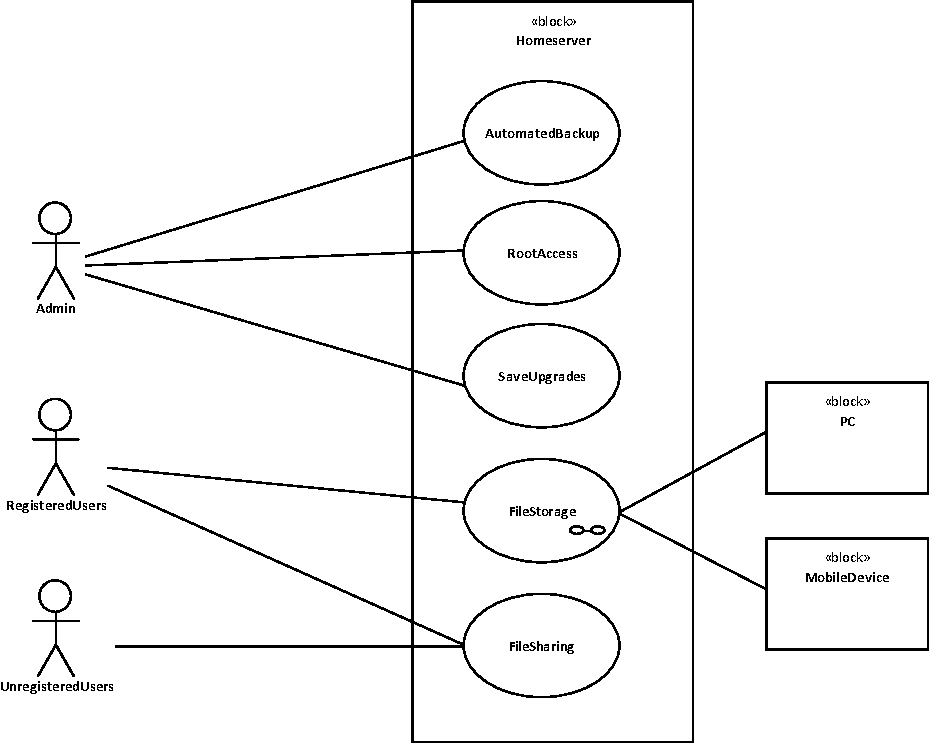
\includegraphics[scale=1]{anford/figures/AnalyseHS}
  \caption[Use-Case-Diagramm Homeserver]{Use-Case-Diagramm der Anforderungen an das System ,,Homeserver'' gegen�ber regestrierten und nicht registrierten Benutzern, sowie dem Administrator und der potentiell einsetzbaren Ger�te}
  \label{fig:analysehs}
\end{figure}

Besonders der Use-Case ,,SaveUpgrade'' war bei der Durchf�hrung des Projektes ein besonderer Schwerpunkt. Die Containervirtualisierung mit Docker erf�llt diese Anforderung. Der Anwendungsfall ,,FileStorage'' l�sst sich noch weiter verfeinern. Das separate Diagramm ist in Abbildung \ref{fig:analysefs} zu finden.

\begin{figure}[h]
  \centering
  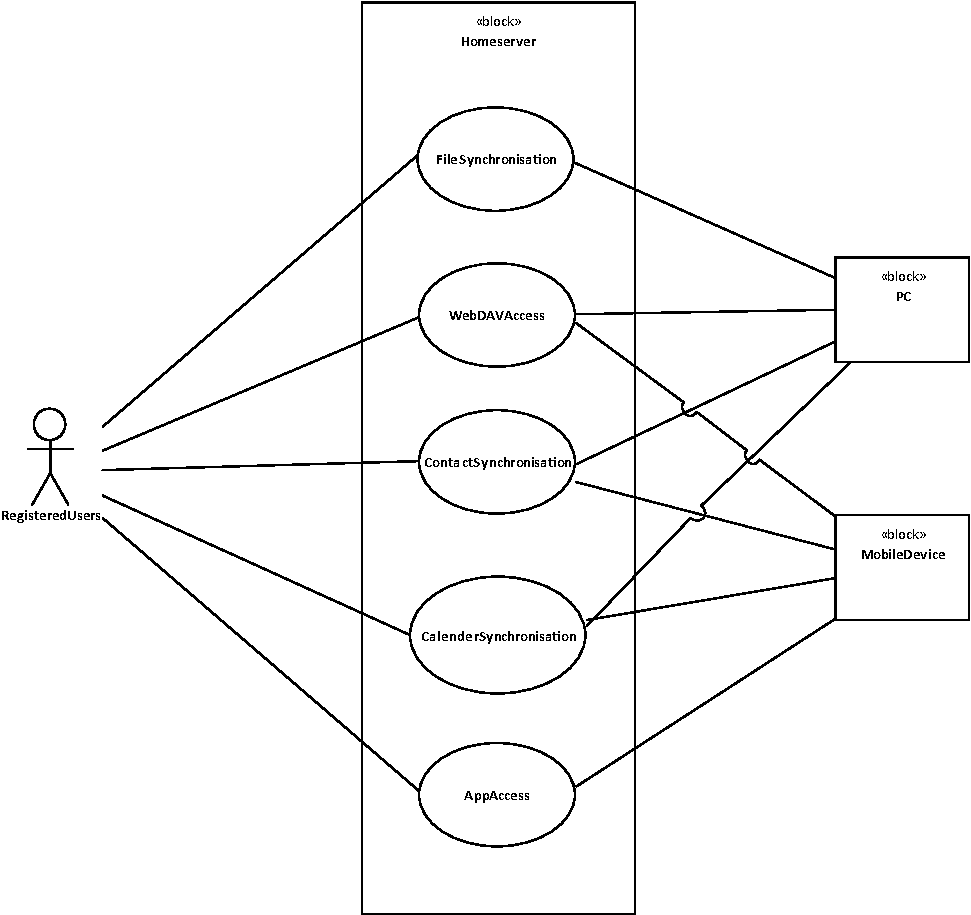
\includegraphics[scale=1]{anford/figures/AnalyseFS}
  \caption[Use-Case-Diagramm File Storage]{Verfeinerung des Anwendungsfalles ,,FileStorage''}
  \label{fig:analysefs}
\end{figure}


%%% Local Variables:
%%% mode: latex
%%% TeX-master: "../doku_server"
%%% End:

\chapter{Projektdurchf�hrung}
\label{sec:details}

\section{Hardware}
\label{sec:hardware}

Die Serverhardware umfasst folgende Komponenten:

\begin{itemize}
\item Fujitsu D3128-B25 Mainboard mit Intel C602 Server Chipsatz
\item 8 x 8 GB DDR3-RDIMM ECC Arbeitsspeicher
\item Intel XEON E5-2560V2 Octa-Core Server-CPU mit Hyperthreading
\item Effizientes \SI{450}{\watt} Modell Straight Power 11 von be quiet!
\item Phanteks Enthoo Pro Tower PC-Geh�use
\item WD-Blue 250 GB SSD Festplatte
\item ARCTIC Freezer 12 CO CPU-K�hler
\item 4 x Seagate ST4000VN008 IronWolf 4 TB HDD Festplatte
\end{itemize}

All diesen Komponenten ist gemeinsam, dass sie auf Server-Anforderungen wie
z.B. Dauerbetrieb optimiert sind. Des Weiteren sind viele der Komponenten
gebraucht sehr g�nstig verf�gbar.

\section{Verwendete Basis-Software}
\label{sec:software}

\subsection{Betriebssystem}
\label{sec:sw_os}

Bevor ein sinnvolles Arbeiten auf dem Server m�glich ist, steht die Entscheidung
f�r ein bestimmtes Betriebssystem und dessen Installation an. Der Autor hat sich
an dieser Stelle f�r den Einsatz eines UNIX-basierten Betriebssystems
entschieden, da f�r solche Systeme die ben�tigte Software frei verf�gbar
ist. Als konkrete Distribution wurde Ubuntu Server 16.04 ausgew�hlt.

Die Installation des Betriebssystems gestaltet sich bei dem gew�hlten Mainboard
etwas aufw�ndiger, weil dieses keine Integrierte Grafikschnittstelle bietet. An
dieser Stelle ergeben sich zwei M�glichkeiten: Entweder es wird zeitweise eine
Grafikkarte verwendet, welche �ber eine PCI-Express Schnittstelle angeschlossen
werden kann, oder es wird eine \textit{vollautomatische} Installation des OS
durchgef�hrt. Im vorliegenden Projekt wurde die letztere Variante
durchgef�hrt. Hierf�r sind folgende Schritte notwendig:

\begin{enumerate}
\item \textbf{Erstellung einer Preseed-Datei:} W�hrend der normalen interaktiven
  Installation werden dem Benutzer verschieden Fragen zur Konfiguration des
  Betriebssystems gestellt. Diese Fragen k�nnen \textit{vor der Installation} in
  einer Datei beantwortet werden. Canonical stellt eine recht umfangreiche
  Dokumentation bereit, wie eine Preseed-Datei zu erstellen ist
  \cite{ubuntu_man_preseeding}. Die in diesem Projekt verwendete
  Preseeding-Datei stammt aus \cite{urbanpenguin_preseeding_wp} und wurde an die
  Bed�rfnisse angepasst.
\item \textbf{Bereitstellung der Datei:} Auch hier gibt es mehrere
  M�glichkeiten: Die Datei kann �ber einen FTP Server, auf dem
  Installationsdatentr�ger oder im initrd bereit gestellt werden. Die
  Bereitstellung �ber FTP bietet sich bei der Installation �ber PXE an. In
  diesem Fall erschien die einfachste M�glichkeit, die Datei auf dem
  Installationsmedium bereit zu stellen. Hierf�r wird z.B. mit dem Programm
  \textbf{Cubic} ein angepasstes ISO-Image erstellt. Die Datei muss dann nur an
  eine beliebige Stelle in dem Image abgelegt werden, wobei sich der Ordner
  ,,preseed'' anbietet.
\item \textbf{Bekanntmachung der Datei f�r den Bootloader:} Der Bootloader muss
  noch erfahren, dass er die Preseed-Datei nutzen soll, anstatt den Benutzer
  nach den Optionen zu fragen. Die folgenden Dateien stellen den Inhalt des
  Men�s dar, welches die Optionen beim starten der Installation entgegen
  nimmt. Der Option ,,Install Ubuntu Server'' wird der Pfad der Preseed-Datei
  mit der Option \texttt{file=/cdrom/path/to/file} hinzu gef�gt. Je nach
  BIOS-Version m�ssen unterschiedliche Dateien editiert werden.
  \begin{itemize}
  \item Legacy: Die Datei \texttt{/isolinux/txt.cfg} muss editiert werden.
  \item UEFI: die Datei \texttt{/boot/grub/grub.cfg} muss editiert werden.
  \end{itemize}
\item \textbf{Weitere Optionen:} Es muss eine Standard-Option mit einem Timeout
  definiert werden, damit die Installation automatisch Startet. In der Datei
  \texttt{/isolinux/txt.cfg} geschieht das �ber den Eintrag \texttt{default
    <label>} und in der Datei \texttt{/boot/grub/grub.cfg} so wie in
  \cite{ubuntuusers_grub2_config} beschrieben. Des Weiteren m�ssen noch die
  Optionen f�r \texttt{locale} z.B. \texttt{en\_us} und
  \texttt{keyboard-configuration/layoutcode} z.B. mit \texttt{us} vorbelegt
  werden, da diese abgefragt werden, \textit{bevor} der Bootloader die
  Preseed-Datei liest, wo diese Optionen ggf. auch spezifiziert wurden.
\end{enumerate}

Es empfiehlt sich, die Installation vorher einmal in einer virtuellen Maschine
zu testen, um festzustellen, ob diese dann auch vollautomatisiert durch
l�uft. Grunds�tzlich sollte die Preseed-Methode auch f�r Ubuntu 18.04
funktionieren \cite{ubuntu_man_preseeding}, jedoch hatte der Autor massive
Probleme mit deren Ausf�hrung und es wurde somit auf Ubuntu 16.04 zur�ck
gegriffen. Ist es unabdingbar eine neuere Distribution zu nutzen, kann nach der
Installation unkompliziert auf die neue Version upgegraded werden.

\subsection{Containervirtualisierung mit Docker}
\label{sec:sw_docker}

Ist die Installation des Betriebssystems �berstanden, er�ffnen sich nun die
Gestaltungs\-m�glichkeiten des eigentlichen Webservers. Dem Autor sind zwei
grunds�tzliche Herangehensweisen bekannt:

\paragraph{,,Harte'' Installation der Komponenten auf der Maschine}

Es ist m�glich, die gew�nschte Software (z.B. einen Webserver, nextcloud,
WordPress usw.) und die ben�tigten Abh�ngigkeiten (z.B. eine
PHP-Laufzeitumgebung) einfach auf der Maschine zu installieren wie jedes andere
Programm auch. Dies allerdings unsch�n im Bezug auf Flexibilit�t und
Wartbarkeit: Nach einiger Zeit ist vergessen, welche Komponenten in welcher
Version installiert wurden. Auch das Upgrade auf neue Versionen ist mit einem
gewissen Risiko verbunden, da nicht mit garantiert werden kann, ob das System
nach dem Upgrade noch so l�uft wie es soll.

\paragraph{Aufteilung der Komponenten in Container}

Die bessere L�sung w�re eine standardisierte Laufzeit- und Entwicklungsumgebung,
die sowohl auf dem Testsystem als auch auf dem Produktivsystem identisch
ist. Genau diese Funktionalit�t stellt Docker bereit: Eine Funktionalit�t wird
in einem \textit{Container} gekapselt. Ein Container ist vergleichbar mit einer
virtuellen Maschine, die jedoch nativ im Kernel des Host-Systems l�uft und
dadurch wesentlich ressourcensparender ist als eine richtige VM. Alle ben�tigten
Abh�ngigkeiten werden zur Laufzeit geladen und sind auch nur dann auf dem System
vorhanden. Sobald der Container nicht mehr ben�tigt wird, kann dieser mit allen
Abh�ngigkeiten mit einem Befehl vollst�ndig entfernt werden.

Des Weiteren kann mit Docker risikofrei ein Versionsupgrade durchgef�hrt werden:
Die neue Version einer Software wird lokal ausgiebig getestet und dann auf das
Produktivsystem geladen. Durch einen Neustart der Container ist das
Versionsupgrade vollzogen und es gibt nicht mal einen Moment Downtime.

Abgesehen von den Linux-Standard-Werkzeugen und einem Editor (der Autor nutzt
GNU (x)Emacs) l�uft s�mtliche Software in Docker-Containern. Die
Server-Software-Architektur ist in Kapitel \ref{sec:sw_arch} beschrieben. 


\section{Softwarearchitektur}
\label{sec:sw_arch}

\subsection{Deployment der Container und der Anwendungen}
\label{sec:sw_arch_depl}


Im Folgenden wird das Deployment der Anwendungen auf dem Server und die interne
Kommunikation der Anwendungen vorgestellt

Wie bereits in \ref{sec:software} angedeutet, werden die Applikationen durch
Kapselung in Docker-Containern organisiert und vom Betriebssystem getrennt.

\begin{figure}[h]
  \centering
  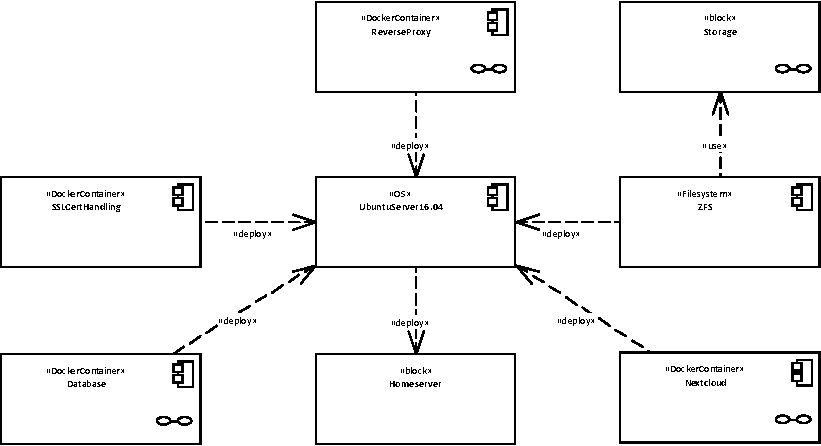
\includegraphics[scale=1]{durchfuehrung/figures/DeploymentOS}
  \caption[Deployment-Diagramm Applikationen und OS]{Komponentendiagramm der
    eingesetzten Softwarekomponenten und ihre Beziehung zum Betriebssystem. Die
    Abh�ngigkeit stereotypisiert mit $\ll$deploy$\gg$ bedeutet hierbei, dass die
    Komponente die jeweilige Ziel\-komponente als Laufzeitumgebung nutzt.}
  \label{fig:deplos}
\end{figure}

\newpage

Das Deployment der Anwendungen selbst erfolgt dann auf die Docker-Container, wie
in Abbildung \ref{fig:depldb} gezeigt. Je nach Konfiguration findet die
Anwendung ein vollst�ndiges Betriebssystem mit allen Abh�ngigkeiten vor, die im
Dockerfile definiert wurden.

\begin{figure}[h]
  \centering
  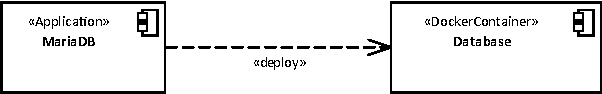
\includegraphics{durchfuehrung/figures/DeploymentDB}
  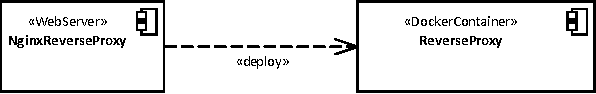
\includegraphics{durchfuehrung/figures/DeploymentRP}
  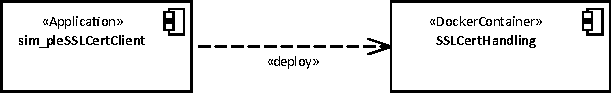
\includegraphics{durchfuehrung/figures/DeploymentSSL}
  \caption[Deployment-Diagramm Anwendungen]{Deployment der Anwendungen auf die
    dazugeh�rigen Docker-Container}
  \label{fig:depldb}
\end{figure}

\newpage
\subsection{Starten der Docker-Container}
\label{sec:sw_arch_start}

Die einfachste M�glichkeit, einen Docker-Container zu starten, ist die Eingabe
des Befehls \texttt{docker run <image\_name>}. Ein Image ist ein mit
\texttt{docker build} gebautes Dockerfile vergleichbar mit dem Image eines
Betriebssystems. Mit dem \texttt{docker run} Befehl wird dieses gestartet und es
entsteht die Instanz eines Images, ein Container. Mehr Informationen zum Befehl \texttt{docker run} ist in \cite{docker_run_reference} zu finden.

Die beschriebene Methode ist f�r einfache Tests gut verwendbar. Ist jedoch ein
komplexes Gebilde aus Containern zu bauen, so ist es nicht zielf�hrend bei jedem
Start alle Container von Hand zu starten. Hierf�r wird von Docker das Werkzeug
Docker Compose bereit gestellt. Dieses liest eine Datei aus (standardm��ig
\texttt{docker-compose.yml}), in der alle Optionen definiert sind, mit denen die
Container sonst mit \texttt{docker run} gestartet werden. Mehr Informationen zu Docker Compose sind in \cite{docker_compose_reference} zu finden.

Im hier vorgestellten System wurde eine \texttt{docker-compose.yml}-Datei f�r
Basisdienste wie die Datenbank und den Reverse Proxy, sowie eine Datei f�r die
konkrete Anwendung wie die Nextcloud. Dieses Verfahren erm�glicht eine getrennte
Verwaltung von Infrastruktur und Anwendung.

\subsection{Interne Kommunikation der Container}
\label{sec:sw_arch_kom}

Um eine Kommunikation zwischen den Containern zu erm�glichen wird das Feature
\textit{network} von Docker genutzt. Dieses erm�glicht den Aufbau virtueller
TCP/IP-Netzwerke innerhalb einer Maschine (=\textit{Bridge}-Netzwerk) oder auch
maschinen�bergreifend (=\textit{Overlay}-Netzwerk) zum Aufbau von Clustern. Da jeder Container eine kleine virtuelle Maschine darstellt, verf�gt auch jeder Container �ber eine Netzwerkschnittstelle, mit der er dem ausgew�hlten Netzwerk beitreten kann.

Im vorliegenden Projekt wurden ausschlie�lich Bridge Netzwerke genutzt, da nur
eine Maschine vorhanden ist. Dabei wurden die Netzwerke \textit{frontend} und
\textit{backend} eingerichtet. Dies erm�glicht eine virtuelle Trennung zwischen
der Benutzerseite (z.B. der Reverse-Proxy, der Nutzeranfragen von au�en
verarbeitet) und dem Server-Backend (z.B. die Datenbank). Abbildung
\ref{fig:compsw} zeigt die Beziehung der Container untereinander.

\begin{landscape}

\begin{figure}[h]
  \centering
  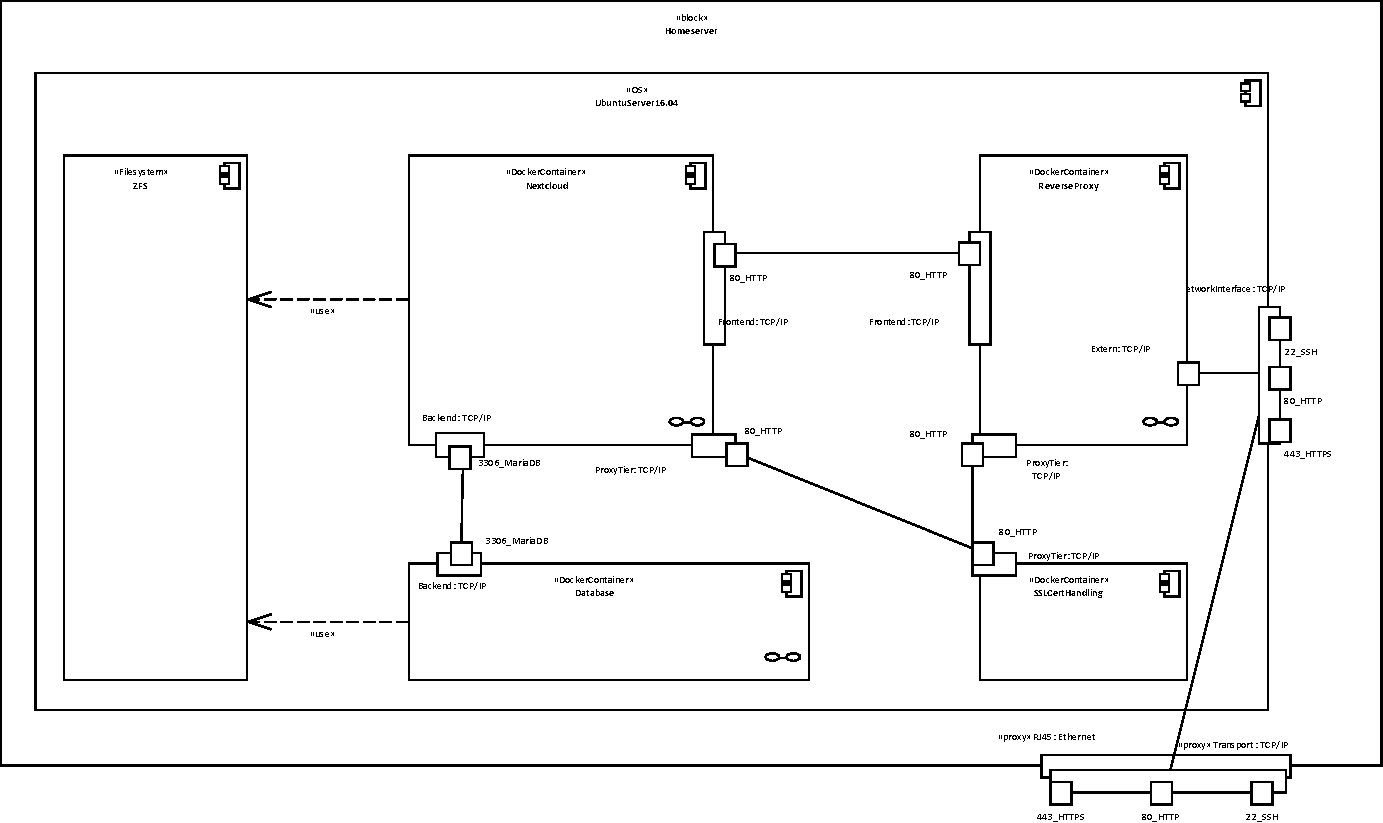
\includegraphics[angle=0, scale=1]{durchfuehrung/figures/CompositionSW}
  \caption[Kompositionsdiagramm der Docker-Container]{Kompositionsdiagramm der eingesetzten Docker-Container. Die Docker-Container sind jeweils �ber die passenden Bridge-Netzwerke \texttt{frontend} und \texttt{backend} miteinander verbunden. Die Datenbank und die Nextcloud nutzen den von ZFS verwalteten Speicherpool als Speicher-Backend}
  \label{fig:compsw}
\end{figure}

\end{landscape}

%%% Local Variables:
%%% mode: latex
%%% TeX-master: "../doku_server"
%%% End:






% \begin{figure}[h]
%   \centering
%   \includegraphics[width=0.6\textwidth, page=5, trim=0cm 0cm 0cm 0cm, clip]{docker_vis.png}q
%   \caption{Docker als Instanz zwischen Applikation und Betriebssytem. \newline Quelle
%     \href{https://www.docker.com/resources/what-container}{\mbox{Docker.com}}}
%   \label{fig:docker}
% \end{figure}


%%% Local Variables:
%%% mode: latex
%%% TeX-master: "../doku_server"
%%% End:






\printbibliography[heading=bibintoc]

\appendix
\chapter{Docker-Compose Dateien}
\label{chap:dockercomp_append}

\begin{longlisting}
  \inputminted{yaml}{append_code/code/docker-compose_base.yml}
  \caption{Docker-compose file f"ur die Datenbank, den Reverse-Proxy und die
    SSL-Zertifikatsverwaltung}
  \label{list:comp_base}
\end{longlisting}

\newpage

\begin{longlisting}
  \inputminted{yaml}{append_code/code/docker-compose_nc.yml}
  \caption{Docker-compose file f"ur die Nextcloud}
  \label{list:comp_nc}
\end{longlisting}

%%% Local Variables:
%%% mode: latex
%%% TeX-master: "../doku_server"
%%% End:



\end{document}


%%% Local Variables:
%%% mode: latex
%%% TeX-master: t
%%% TeX-command-extra-options: "-shell-escape"
%%% End:
